\chapter{Discussion ESB in Openshift}
\label{cha:esbd}
This chapter will evaluate the implemented prototype of Chapter \vref{cha:esbi}, and will show that challenges such as
\begin{itemize}
	\item managing multiple environments,
	\item managing multiple service versions,
	\item managing public API migration,
	\item managing adapters and transformers as services,
	\item and managing service security
\end{itemize}
are manageable tasks when hosting an ESB in Openshift. Whenever possible, Openshift will be compared to JBoss EAP, which is used as the platform for ESB middleware as discussed in Section \vref{fig:esb-software-architecture}.

\section{Managing Multiple Environments}
\label{sec:esbd-multiple-env}
An ESB is commonly hosted on multiple environments, whereby at least one productive and one testing environment should be present. These environments where commonly a VM, which provides the runtime environment for the ESB. As the prototype shows, the environment is now represented by an Openshift Project, which can be reproduced easily via scripts as discussed in Section \vref{sec:esbi-openshift}. \\

The services hosted on the ESB are using Fuse integration Service 2.0 and its provided tooling, which ensure that the services are properly encapsulated in a container and properly managed in Openshift. Therefore, the service developers provide the necessary Openshift Templates, which has the effect, that the operators have no interaction with the service artifacts and runtime environments anymore. Operator have only to manage
\begin{itemize}
	\item the Openshift Project, which hosts the services,
	\item the Openshift ConfigMaps, which hold the service non-sensitive configuration,
	\item the Openshift Secrets, which hold the sensitive service configuration,
	\item and scripts for utility such as backup/restore of service data or instance scaling.
\end{itemize} 
\ \\
Listing \vref{ls:esboi-config-project-stages-prod} shows how developers reference Openshift Objects such as Openshift ConfigMaps and Openshift Secrets, which are managed by operators. 

Figure \vref{fig:esbd-multi-stage-env} illustrates the management and provisioning of multiple environments for an ESB, whereby the hosting environment is represented by an Openshift Project. The \mentionedtext{Management Server} pulls the scripts and Openshift Templates from a \mentionedtext{VCS Server} and the configurations from a \mentionedtext{Configuration Server}, and uses them to provision new Openshift Projects or manage existing ones. \\

The scripts and Openshift Templates are separated from the configurations, which are actually providing the data for the scripts and Openshift Template-Parameters. With such an approach, the infrastructure becomes reproducible, versioned, and therefore consistent, and disposable. These characteristics are also principles of IaC, which have been discussed in Chapter \vref{cha:iac}. 

\begin{figure}[htbp]
	\centering
	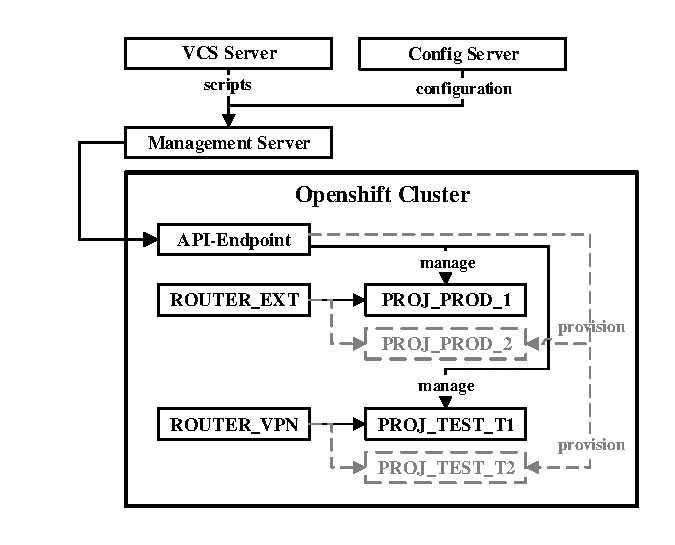
\includegraphics[scale=1]{images/esbd-multi-stage-env.pdf}
	\caption{Management and provisioning of multiple environments}
	\label{fig:esbd-multi-stage-env}
\end{figure}

The interaction of the \mentionedtext{Management Server, VCS Server} and \mentionedtext{Configuration Server} as illustrated in Figure \vref{fig:esbd-multi-stage-env}, is similar to the Figure \vref{fig:reproduce-infrastructure}, which illustrated how a system can be reproduced with parametrized templates and an IaC tool. The Openshift CLI provides functionality to manage Openshift Objects, which is what needs to be done when providing an environment in form of an Openshift Project, therefore the Openshift CLI acts as an IaC tool.  \\

The Feature Table \vref{tab:esbd-multi-stage-env} illustrates what mechanisms Openshift and JBoss EAP contain to provide the listed features. As illustrated in the table, Openshift provides \mentionedtext{Networking} and \mentionedtext{Isolation} features, which are provided to JBoss EAP by its hosting environment, such as a VM. Except of the \mentionedtext{Networking} and \mentionedtext{Isolation} feature, JBoss EAP supports all other features either natively or by supporting a third party framework. Nevertheless, Openshift combines all features in one platform, and makes them easy manageable via Openshift Templates and the Openshift CLI.

{\renewcommand{\arraystretch}{1.2}%
\begin{table}[h]
	\begin{tabularx}{\textwidth}{ X|c|c }	
	  \textbf{Feature}              & \textbf{Openshift}      & \textbf{JBoss EAP} \\  \hline
	  \textit{Staging}                  & Openshift Project       & Server Instance \\  \hline
	  \textit{Management}               & Openshift CLI           & JBoss CLI \\
	                                    & Openshift Web-Console   & JBoss Web-Console \\
	                                    & Openshift REST-API      & \\  \hline
	  \textit{Networking}               & Openshift Project-Network & none (VM) \\
	                                    & Openshift Service       & \\  
	                                    & Openshift Route         & \\  \hline
	  \textit{Isolation}                & Openshift Project       & none (VM) \\  \hline
	  \textit{Configuration/Secrets}    & Openshift ConfigMaps    & Java System Properties  \\
	                                    & Openshift Secrets       & Environment variables \\
	                                                             && Password Vault \\  \hline
	  \textit{Service Distribution}     & Openshift Worker-Node   & Single JVM \\ 
			                                                     && Karaf \\  
			                                                     && OSGI \\  \hline
	  \textit{Roll-out}                 & Recreate                & Framework dependent, \\ 
			                            & Rolling                 & normally recreate \\
			                            & Blue/Green              & \\  \hline
	\end{tabularx}
	\caption{Feature comparison between Openshift and JBoss EAP}
	\label{tab:esbd-multi-stage-env}
\end{table}}

\section{Managing Multiple Service Versions}
\label{sec:esbd-multi-version-service}


\section{Managing Migration of Public API}
\label{sec:esbd-multi-stage-env}

\section{Managing Adapters and Transformers as Services}
\label{sec:esbd-adap-trans-service}

\section{Managing Service Security}
\label{sec:esbd-service-security}

\section{Further Work}
\label{sec:esbd-furhter-work}